\documentclass[letterpaper]{article}
\usepackage[submission]{aaai2027}
\usepackage[hyphens]{url}
\usepackage{graphicx}
\usepackage{tikz}
\usetikzlibrary{arrows.meta, positioning, fit, calc, shapes.geometric}
\usepackage{microtype}
\usepackage{natbib}
\urlstyle{rm}
\def\UrlFont{\rm}
\usepackage{caption}
\frenchspacing
\usepackage{amsmath}
\usepackage{amssymb}
\usepackage{booktabs}
\usepackage{multirow}
\usepackage{cuted}
\emergencystretch=1.2em
\pdfinfo{
/TemplateVersion (2027.1)
}
\setcounter{secnumdepth}{0}

\title{WEAVE: Wavelet-Decoupled Velocity Matching for Lightweight Style Transfer}
\author{Anonymous Submission}
\affiliations{}
\begin{document}
\maketitle

\begin{abstract}
For style transfer, SOTA diffusion models and training-free variants built on them exceed the VRAM limits of consumer GPUs. Meanwhile, lightweight alternatives can underperform a trivial identity mapping (copying the source), which scores high on traditional metrics but is rarely evaluated as a baseline. We trace this to frequency dominance in shared representation spaces: low-frequency structural energy overwhelms high-frequency style gradients and can push optimization toward identity-like solutions.

We argue that an effective method must outperform this identity baseline while remaining computationally affordable. To
this end, we propose WEAVE, a wavelet-decoupled framework operating in the VAE latent space. A single-level Haar transform splits the latent into a low-frequency structure band, where a lightweight velocity model handles source-aligned transport, and high-frequency style bands where stepwise statistical alignment injects target style. This decoupling separates content transport from style injection, letting WEAVE train in under two minutes on a single consumer GPU.

We also advocate the IDT--TGT sandwich as an evaluation guideline. IDT returns the source unchanged, while TGT returns an unrelated image from the target style; together they contextualize valid transfer. Under this guideline, WEAVE exceeds the identity reference on the reported board with 1.04M trainable parameters (plus a frozen 84M VAE).
\end{abstract}

\begin{strip}
\noindent
\includegraphics[width=\textwidth]{fig_distinct5_page1_summary.pdf}
\captionof{figure}{IDT--TGT sandwich comparison on Distinct5-WikiArt.
Left: the two axes represent style affinity and content preservation; bubble area denotes training time and red marks WEAVE. IDT and TGT provide the displayed style and content references. Right: target-pooled ArtFID on the same benchmark. IDT shows the board estimate and a 95\% target-style bootstrap interval; TGT shows the mean and 2.5--97.5 percentile interval over 30 reference draws. Bar labels give training time.}
\label{fig:page1}
\end{strip}

\section{Introduction}

Style transfer faces two linked problems in deployment and evaluation. Recent image
foundation models such as Qwen-Image and FLUX.2 provide strong generation and editing
priors~\cite{wu2025qwenimagetechnicalreport,blackforestlabs2025flux2}, but can require
more than 60\,GB of GPU memory. Lightweight alternatives
avoid this cost, but some preserve the source so strongly that their style affinity falls
below the unchanged input. Conventional protocols can hide this no-op behavior: LPIPS rewards
source reconstruction, and the content factor of ArtFID can favor a near-copy, yet the
identity mapping is rarely reported as an explicit baseline.

Figure~\ref{fig:page1} makes the missing comparison visible with two simple outputs.
Identity (IDT) returns the source unchanged, while Target Style (TGT) returns an unrelated
reference from the requested style. A useful transfer should move beyond IDT in the style
direction without moving as far from the source as TGT in the content direction. The two
references expose opposite failures in the original metric units: methods below IDT have
not acquired enough target style, whereas methods beyond TGT have discarded at least as
much source content as a source-independent style image. We call this the IDT--TGT sandwich.
We report this diagnostic alongside DINO, CLIP, LPIPS, and visual comparisons.

Why do compact models enter the identity regime? Our probes identify the shared coordinate
system as one contributor, separate from parameter count. Neural networks learn low
frequencies first~\cite{rahaman2019spectral,xu2022frequency}, and natural images place much
more energy in global layout and object shape than in brushstroke and fine texture. A
velocity model trained on the full latent must explain both with one field.
The resulting low-frequency residuals are larger and easier to fit, so their gradients
dominate the update and weaken style-conditioned high-frequency motion. Frequency-domain
translation reports a related content--style conflict~\cite{cai2021fdit}; our gradient and
subband probes measure it directly in the trained model. Simply increasing width does not
change this competition because both signals still share the same basis and objective.

We therefore propose WEAVE, which changes the representation and target before increasing
capacity. A frozen diffusion VAE supplies a compact latent, while a one-level Haar transform
separates low-frequency structure (LL) from oriented texture (LH/HL/HH). A 1.04M-parameter
velocity model learns source-aligned transport with weaker LL supervision; compact
orientation-specific target codes modulate the matching LH/HL heads; and one
stepwise AdaIN update supplies target-style statistics to the high-frequency residual. Cached
latents remove the VAE encoder and diffusion U-Net from training; eight compact Euler
evaluations and one VAE decode are sufficient at inference. An internal gradient transition
selects the fourth epoch without image evaluation, giving a 1.4-minute run on one RTX~3060;
the same Haar statistical operator can be added to a frozen SD1.5 editor without retraining.

\paragraph{Contributions.}
(1)~\textbf{Evaluation:} We advocate the IDT--TGT sandwich, which reports a no-op reference
and a source-independent target-style reference alongside standard metrics, exposing both
style suppression and content collapse.
(2)~\textbf{Representation and method:} We measure low-frequency gradient dominance in a
shared latent objective and develop a wavelet-decoupled transport that assigns structure,
learned texture transport, and trajectory-level statistics to explicit paths.
(3)~\textbf{Efficiency and evidence:} WEAVE uses 1.04M trainable parameters and 1.4 minutes of
single-GPU training. Cross-dataset evaluation, internal gradient probes, and a frozen
SD1.5 plugin provide empirical checks beyond the main board.
\begin{figure*}[t!]
\centering
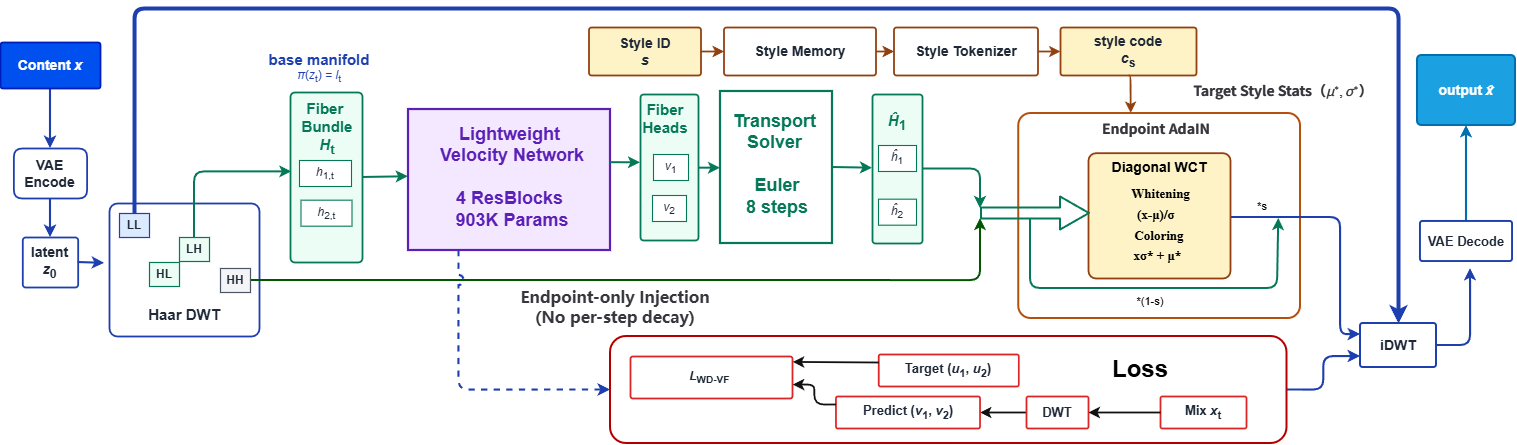
\includegraphics[width=\textwidth]{aaai_arch_diagram_v16_staggered_bundle.drawio.png}
\caption{\textbf{WEAVE architecture}. A single-level Haar transform exposes LL and three
high-frequency bands. The compact velocity network predicts LL/LH/HL motion, while pooled
target LH/HL codes modulate their matching residual heads; HH has no learned velocity head.
After every Euler update, high-frequency AdaIN aligns the combined high-frequency residual to
the target-style statistics. The complete D5 model has 1.04M trainable parameters.}
\label{fig:framework}
\end{figure*}
\section{Related Work}
\label{sec:related}

\subsection{Neural Style Transfer}
\label{sec:rw-nst}
Artistic style transfer was introduced by optimizing pixels to match content features and
Gram statistics of a pretrained network~\cite{gatys2015neural,gatys2016image}. AdaIN
aligns channel-wise moments~\cite{huang2017arbitrary}, while WCT aligns a full feature
covariance~\cite{li2017universal}; both replace iterative optimization with a feed-forward
feature transform. SANet and transformer-based variants add correspondence or long-range
attention~\cite{park2019sanet,deng2022stytr2,hong2023aespa,kwon2024aesfa}, and CUT learns
unpaired translation through patch-level contrast~\cite{park2020cut}. Training-free methods
also reuse pretrained codebooks or hierarchical vision transformers~\cite{gim2024cast,zhang2024s2wat}.
The survey of Zhang et al.~\cite{zhang2025survey} summarizes this progression. These methods
differ in supervision and backbone, but most still mix structure and appearance in one
feature tensor. Stronger moment or attention transfer can therefore alter source geometry;
WEAVE instead restricts the analytic style correction to explicit frequency coordinates.

\subsection{Diffusion-based and Training-free Style Editing}
\label{sec:rw-diffusion}
Latent diffusion models~\cite{rombach2022high} move editing into a compressed generative
space and provide strong semantic priors. Prompt-to-Prompt and SDEdit control generation
through attention or noising~\cite{hertz2022prompt,meng2021sdedit}; StyleID and StyleAligned
modify attention statistics~\cite{chung2024style,hertz2024style}; IP-Adapter adds an image
prompt~\cite{ye2023ipadapter}; and InST, DiffuseIT, ArtBank, and Z-STAR use inversion or
pretrained features for style transfer~\cite{zhang2023inst,kim2022diffuseit,zhang2024artbank,lu2024zstar}.
These methods are often called training-free because they do not update backbone weights,
but inference still invokes a large denoiser repeatedly and may require inversion. Recent
Qwen-Image and FLUX.2 illustrate the resulting deployment gap between large image
backbones and compact transfer models~\cite{wu2025qwenimagetechnicalreport,blackforestlabs2025flux2}.
WEAVE retains only the frozen VAE and learns the remaining transport with a compact model;
the SD1.5 plugin separately tests whether the analytic Haar operator transfers back to
a large pretrained editor.

\subsection{Flow Matching and Schr\"odinger Bridges}
\label{sec:rw-sb}
Rectified flow~\cite{liu2022rectified} and flow matching~\cite{lipman2022flow} regress a
velocity along an interpolation between endpoint distributions, enabling short numerical
paths. Schr\"odinger bridges~\cite{leonard2014survey} add entropy-regularized stochastic
transport, and DSB, DSBM, I2SB, and DDIB develop practical diffusion or flow solvers for
unpaired domains~\cite{debortoli2021dsb,shi2023dsbm,liu2023i2sb,su2023ddib}. These methods
are related to regularized optimal transport~\cite{cuturi2013sinkhorn,peyre2019computational},
but their image objectives usually measure all coordinates together.
WEAVE uses endpoint-interpolation velocity regression with a source-aligned endpoint,
an orthogonal wavelet basis, and separately weighted blocks. This retains a short numerical
trajectory while changing which errors compete during learning.

\subsection{Lightweight Models and Evaluation}
\label{sec:rw-light}
Mamba-based SaMST and SaMam reduce trainable size and sequence cost~\cite{liu2024samst,liu2024samam,gu2023mamba},
showing that style transfer need not inherit a full diffusion U-Net. Efficiency alone,
however, does not establish that the output moved toward the requested style. LPIPS
measures perceptual source distance~\cite{zhang2018unreasonable}, and ArtFID combines style
distribution and content terms~\cite{wright2022artfid}; both can reward a near-copy when the
identity output is omitted.
IDT makes this no-op score explicit. TGT adds the opposite reference: a target-style image
with no source dependence. Reporting both rows preserves the standard metrics and their raw
units, while identifying whether an apparent gain comes from style suppression or content
collapse. The references are benchmark-specific diagnostics rather than universal thresholds.

\subsection{Spectral Bias and Frequency-aware Optimization}
\label{sec:rw-spectral}
Neural networks preferentially fit low-frequency functions~\cite{rahaman2019spectral,xu2022frequency},
and natural images place most spectral energy in coarse structure. The two effects are
distinct but reinforce each other: the training target supplies larger low-frequency
residuals, while the network fits those residuals earlier. Frequency-domain translation
therefore constrains low and high frequencies separately to protect content identity~\cite{cai2021fdit}.
FreqFlow instead introduces time-dependent frequency weighting and a dedicated frequency
branch for class-conditional flow-based image generation~\cite{ren2026freqflow}.
Our contribution is to examine this optimization imbalance in a compact velocity model through
per-band loss, input gradients, head
gradients, and endpoint interventions. The measurements motivate a structural preconditioner
for source-conditioned, unpaired style transfer rather than unconditional generation.

\subsection{Wavelet and Latent-space Alignment}
\label{sec:rw-wavelet}
Wavelets separate local information by scale and orientation and support exact
reconstruction. They have been used in restoration and generation~\cite{phung2023wavelet}
and in photorealistic style transfer~\cite{yoo2019photorealistic}. The Haar basis is
particularly simple: its orthogonality gives additive energy decomposition, and its compact
support preserves local correspondence~\cite{daubechies1992ten}. VAE latents provide a
complementary reduction in spatial cost~\cite{rombach2022high}, while AdaIN and WCT provide
closed-form statistical alignment.
WEAVE combines these ingredients inside the transport objective rather than using wavelets
only as preprocessing or postprocessing. LL, LH, and HL receive explicit velocity roles;
HH is handled only by stepwise statistical alignment. This division is the central difference from a
single latent-space transform such as Latent-WCT.



\section{Method}
\label{sec:method}

A direct content-to-style target changes layout, palette, and texture at once. Under shared
latent MSE, the largest residual can dominate the update even when it is not the most useful
signal for style transfer. WEAVE instead constructs a low-frequency-aligned target, learns
band-weighted transport, and corrects high-frequency statistics along the inference path
(Figure~\ref{fig:framework}).

\subsection{Why Split the Transport}
\label{sec:mechanism}

In a shared latent objective, coarse structural residuals and style residuals compete for the
same capacity. Our probes show larger LL transport energy and shared-trunk gradients, while
style separation is stronger in high-frequency bands (Figure~\ref{fig:frequency-probes}).
WEAVE therefore changes the LL target, assigns separate output heads, and downweights---but
does not remove---the LL regression term. The resulting design follows the measured
optimization imbalance in this model.





\subsection{Framework Setup}
\label{sec:framework}

Let $z_c=\mathcal E(x_c)\in\mathbb R^{4\times H\times W}$ and
$z_s=\mathcal E(x_s)$ be content and target-style latents from the frozen SD1.5
VAE~\cite{rombach2022high}. A direct path from $z_c$ to $z_s$ also learns the unrelated
geometry of $x_s$. We instead decompose
$\mathcal W(z_c)=(\ell_c,h_{1,c},h_{2,c},h_{3,c})$ and similarly for $z_s$, then form
the low-frequency-aligned endpoint
\begin{equation}
\begin{aligned}
\tilde\ell_s &=(1-\alpha)\ell_c+
\alpha\,\mathrm{AdaIN}(\ell_c,\ell_s),\qquad \alpha=0.3,\\
z_1^\star&=\mathcal W^{-1}(\tilde\ell_s,h_{1,s},h_{2,s},h_{3,s}).
\end{aligned}
\label{eq:aligned-target}
\end{equation}
The LL blend scales the supervised coarse movement while retaining the source coordinate as
its anchor; the high-frequency target comes from the requested style. Exact source LL suppresses palette
change, whereas the complete style latent would also supervise unrelated target geometry.

Thus $\alpha$ scales the supervised coarse movement, while the target high-frequency bands
retain an appearance signal. This target construction is distinct from reducing the LL loss
weight: the former changes the requested velocity and the latter changes its optimization
pressure.

Training samples a lightly perturbed endpoint interpolation
\begin{equation}
z_t=(1-t)z_c+t z_1^\star-\sigma\sqrt{t(1-t)}\,\epsilon,\qquad
u=z_1^\star-z_c,
\label{eq:rf-path}
\end{equation}
where $t\sim\mathcal U([0,1])$, $\epsilon\sim\mathcal N(0,I)$, and $\sigma=0.02$.
The perturbation regularizes the input state and vanishes at both endpoints; the supervision
remains the clean endpoint displacement $u$. At inference, the perturbation is absent.
Because $\mathcal W$ is linear, the interpolation decomposes into the same subbands. WEAVE
changes the endpoint construction, parameterization, and frequency weights of this velocity
regression.

\subsection{Wavelet Decomposition and Frequency Routing}
\label{sec:wavelet}

\paragraph{Haar wavelet decomposition.}
A one-level Haar transform gives $\mathcal W(z_t)=(\ell_t,h_{1,t},h_{2,t},h_{3,t})$: one
LL band and three high-frequency bands. Haar is orthonormal, local, and exactly invertible,
which lets us assign losses and prediction heads to explicit coordinates
~\cite{daubechies1992ten}. This separation is exact in latent space, although the nonlinear
VAE decoder can still couple visible color, texture, and structure.
For each $2{\times}2$ latent block $(a,b,c,d)$, our transform is
\begin{equation}
\begin{bmatrix}\ell\\h_1\\h_2\\h_3\end{bmatrix}
=\frac{1}{2}
\begin{bmatrix}
1&1&1&1\\1&1&-1&-1\\1&-1&1&-1\\1&-1&-1&1
\end{bmatrix}
\begin{bmatrix}a\\b\\c\\d\end{bmatrix}.
\label{eq:haar-block}
\end{equation}
The rows are orthonormal, so the transform preserves energy and the inverse is its
transpose. LL records the block average; LH, HL, and HH record vertical, horizontal, and
diagonal changes, respectively. This is the precise sense in which WEAVE ``separates
frequencies''; it does not assume that each band contains only one semantic factor.

\paragraph{Affine-fiber view.}
For $\mathcal W(z)=(\ell_z,h_{1,z},h_{2,z},h_{3,z})$, define
$P_Lz=\mathcal W^{-1}(\ell_z,0,0,0)$ and $P_H=I-P_L$. Let $\mathcal Z_L$ be the
range of $P_L$ and $\mathcal Z_H=\ker P_L$ its orthogonal complement. Haar gives the direct sum
$\mathcal Z=\mathcal Z_L\oplus\mathcal Z_H$. For a fixed low-frequency coordinate $\ell$,
the corresponding affine fiber is
\begin{equation}
\mathcal F_\ell=\{z:P_Lz=\ell\}
=\mathcal W^{-1}(\ell,0,0,0)+\mathcal Z_H.
\label{eq:affine-fiber}
\end{equation}
Latents in $\mathcal F_\ell$ share the same Haar LL coordinate but may differ in local
appearance after decoding. WEAVE does not keep $\ell$ exactly fixed: the aligned target and the
$\lambda_{LL}=0.3$ loss allow a limited coarse-color motion. In contrast, the stepwise
AdaIN operator acts on $P_Hz$ and then reattaches the current low-pass component. We use
``fiber'' for this exact affine decomposition.

\paragraph{Empirical frequency probes.}
Across 5,000 cross-style latent pairs, transport energy concentrates in LL while style separation is strongest in HH (Figure~\ref{fig:frequency-probes}). This motivates a weak LL loss and greater emphasis on high-frequency prediction.

\begin{figure}[t]
\centering
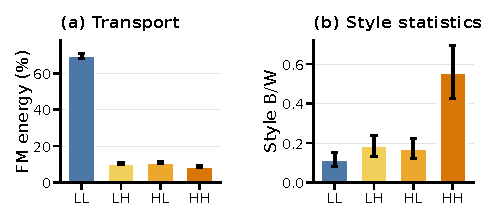
\includegraphics[width=0.98\columnwidth]{fig_probe_combined.pdf}
\caption{\textbf{Frequency probes.} (a) Share of cross-style endpoint-displacement energy in each Haar band. (b) Between-style/within-style variance ratio of per-image latent statistics. Error bars show the standard error across source--target style routes in (a) and across style families in (b).}
\label{fig:frequency-probes}
\end{figure}

\begin{figure*}[t!]
\centering

\includegraphics[width=\textwidth]{fig_teaser_comparison.png}
\caption{Extreme cross-domain stylization (Minimalism $\to$ Rococo). Diffusion editors
substantially alter source structure, while several lightweight or classical outputs remain
close to identity. WEAVE retains the source topology while adding the target's painterly
appearance.}
\label{fig:teaser}
\end{figure*}

\paragraph{Architecture.}
The velocity network uses four width-64 residual blocks and separate $1{\times}1$ heads
for LL, LH, and HL. Pooled LH/HL codes modulate only their matching heads, preserving
target appearance without passing target coordinates into the LL path. WEAVE does not learn
an HH velocity head; HH is handled by the statistical update below.

\paragraph{Why it trains quickly.}
Each pair provides a direct endpoint displacement at every sampled time, while
stepwise AdaIN supplies high-frequency moments analytically. Training therefore regresses a
small latent-space velocity field rather than unrolling a denoiser, inversion, or adversarial
game. The frozen VAE, cached latents, and eight-step solver account for the measured cost.

\paragraph{Spectral velocity-matching objective.}
Let $(v_\ell,v_{h_1},v_{h_2})=v_\theta(z_t,t,s)$ denote the bandwise velocity predicted
from the current latent, time, and target-style condition, and let
$(u_\ell,u_{h_1},u_{h_2},u_{h_3})=\mathcal W(u)$. The spectral velocity-matching term is
\begin{equation}
\begin{aligned}
\mathcal L_{\mathrm{SFM}}:=\mathbb E_t\big[&
\lambda_{LL}\|v_\ell-u_\ell\|_2^2
+\|v_{h_1}-u_{h_1}\|_2^2\\
&+\|v_{h_2}-u_{h_2}\|_2^2\big],
\end{aligned}
\label{eq:weave-loss}
\end{equation}
with $\lambda_{LL}=0.3$. The lower LL weight limits structural
dominance while still allowing coarse tone to move.
The distinct output heads remove output-level sharing, while the common trunk can still
couple the bands. HH is omitted because WEAVE has no HH velocity head. The ablation in
Table~\ref{tab:ablation} shows similar performance with $\lambda_{LL}=1.0$.

\subsection{Stepwise High-frequency Statistical Alignment}
\label{sec:eota}

Velocity matching organizes LL/LH/HL motion but leaves a weak appearance signal. WEAVE
therefore applies AdaIN to the combined high-frequency residual after every Euler
update. Using the projections defined above, for a current residual
$q=P_H(z)$ and target residual $q_s=P_H(z_s)$, define~\cite{huang2017arbitrary}
\begin{equation}
\mathcal A(q;q_s)=
\frac{q-\mu(q)}{\sigma(q)}\,\sigma(q_s)+\mu(q_s),
\label{eq:spatial-fiber-adain}
\end{equation}
where $\mu$ and $\sigma$ are channel-wise spatial statistics. One inference step is
\begin{equation}
\begin{aligned}
\bar z^{k+1}&=z^k+\frac{1}{K}\,\mathcal W^{-1}
\big(v_\ell^k,v_{h_1}^k,v_{h_2}^k,0\big),\\
z^{k+1}&=P_L(\bar z^{k+1})+(1-\beta)q^{k+1}
+\beta\,\mathcal A(q^{k+1};(1+\eta)q_s),
\end{aligned}
\label{eq:stepwise-alignment}
\end{equation}
with $q^{k+1}=P_H(\bar z^{k+1})$, $K=8$, $\beta=2.0$, and $\eta=0.1$ in our experiments.
Since $\beta>1$, the update extrapolates from the current residual toward the
matched target statistics. Applying it at every step makes statistical alignment part of
the inference dynamics rather than a post-processing operation. The learned LH/HL path
provides organized motion, while the same update supplies statistics to HH. The matched
control confirms that removing AdaIN moves the result toward source preservation.


\subsection{Training and Inference}

Training minimizes Eq.~\ref{eq:weave-loss}. Inference uses eight Euler steps and the frozen
VAE decoder. Optimization, caching, probe, and evaluation settings are given in the
supplement.



\section{Experiments}
\label{sec:exp}

\begin{table*}[t!]
\centering
\footnotesize
\renewcommand{\arraystretch}{0.9}
\setlength{\tabcolsep}{0pt}
\resizebox{\textwidth}{!}{%
\begin{tabular}{@{}lccccccccccccccc@{}}
\toprule
Method & \multicolumn{4}{c}{D5-512} & \multicolumn{4}{c}{P2A-256} & \multicolumn{4}{c}{R5-WikiArt} & Params & Train & Infer \\
\cmidrule(lr){2-5} \cmidrule(lr){6-9} \cmidrule(lr){10-13} \cmidrule(lr){14-14} \cmidrule(lr){15-15} \cmidrule(lr){16-16}
& DINO-S$\uparrow$ & CLIP-S$\uparrow$ & LPIPS$\downarrow$ & DINO-C$\uparrow$ & DINO-S$\uparrow$ & CLIP-S$\uparrow$ & LPIPS$\downarrow$ & DINO-C$\uparrow$ & DINO-S$\uparrow$ & CLIP-S$\uparrow$ & LPIPS$\downarrow$ & DINO-C$\uparrow$ & M & min & 750 imgs \\
\midrule
Identity & 0.419 & 0.693 & 0.000 & 1.000 & 0.416 & 0.663 & 0.000 & 1.000 & 0.433 & 0.731 & 0.000 & 1.000 & 0 & free & 0\,s \\
Target Style & 1.000 & 0.863 & 0.776 & 0.215 & 1.000 & 0.835 & 0.800 & 0.169 & 1.000 & 0.796 & 0.747 & 0.230 & 0 & free & 0\,s \\
SD-Turbo & 0.484 & 0.693$^{\dagger}$ & \underline{\underline{\textbf{0.003}}} & \underline{\underline{\textbf{0.922}}} & 0.341$^{\dagger}$ & 0.674 & 0.603 & 0.279 & 0.505 & 0.767 & 0.449 & 0.538 & 0$^{+1100}$ & free & 5\,m \\
StyleAligned & \underline{\underline{\textbf{0.675}}} & 0.780 & 0.869$^{\ddagger}$ & 0.239 & \underline{\underline{\textbf{0.612}}} & 0.768 & 0.786 & 0.310 & \underline{\underline{\textbf{0.649}}} & \underline{\underline{\textbf{0.824}}} & 0.829$^{\ddagger}$ & 0.315 & 0$^{+1100}$ & free & 77\,m \\
Z-STAR & 0.449 & 0.784 & 0.347 & 0.549 & 0.514 & \underline{\underline{\textbf{0.786}}} & 0.332 & 0.526 & 0.514 & \underline{\textbf{0.822}} & 0.384 & 0.526 & 0$^{+1100}$ & free & 3\,h\\
StyleShot & \underline{\textbf{0.563}} & \underline{\textbf{0.787}} & 0.765$^{\ddagger}$ & 0.377 & \underline{\textbf{0.552}} & \underline{\textbf{0.774}} & 0.713 & 0.335 & 0.484 & 0.787 & 0.795$^{\ddagger}$ & 0.380 & 0$^{+2400}$ & free & 5.1\,h \\
StyleID & 0.548 & \underline{\underline{\textbf{0.822}}} & 0.552 & 0.416 & 0.256$^{\dagger}$ & 0.648$^{\dagger}$ & 0.691 & 0.147$^{\ddagger}$ & \underline{\textbf{0.571}} & 0.815 & 0.493 & 0.374 & 0$^{+1100}$ & free & 63\,m \\
CUT & 0.471 & 0.714 & 0.374 & 0.795 & 0.539 & 0.754 & 0.494 & 0.702 & 0.441 & 0.710$^{\dagger}$ & 0.620 & \underline{\textbf{0.795}} & \underline{\textbf{7.0}} & 322.6 & 5\,m \\
SaMST & 0.271$^{\dagger}$ & 0.618$^{\dagger}$ & 0.749$^{\ddagger}$ & 0.145$^{\ddagger}$ & 0.501 & 0.709 & 0.398 & 0.838 & 0.461 & 0.667$^{\dagger}$ & 0.612 & 0.615 & 8.3 & \underline{\textbf{39.5}} & 10\,m \\
SaMam & 0.477 & 0.582$^{\dagger}$ & \underline{\textbf{0.243}} & \underline{\textbf{0.812}} & 0.505 & 0.677 & \underline{\underline{\textbf{0.205}}} & \underline{\underline{\textbf{0.870}}} & 0.503 & 0.712$^{\dagger}$ & \underline{\underline{\textbf{0.227}}} & \underline{\underline{\textbf{0.925}}} & 8.8 & 436.0 & 17.6\,m \\
StyTR-2 & 0.501 & 0.709 & 0.596 & 0.747 & 0.515 & 0.722 & 0.495 & 0.555 & 0.533 & 0.759 & 0.553 & 0.737 & 35.4$^{+12.9}$ & $\sim$1440$^{\ast}$ & 38\,m \\
AesPA-Net & 0.520 & 0.724 & 0.548 & 0.601 & 0.498 & 0.744 & 0.571 & 0.522 & 0.545 & 0.782 & 0.409 & 0.728 & 11.3$^{+20.0}$ & -- & 23\,m \\
Seedream 4.5 & 0.486 & 0.720 & 0.477 & 0.739 & 0.517 & 0.752 & \underline{\textbf{0.227}} & 0.785 & 0.504 & 0.742 & 0.486 & 0.725 & -- & API & -- \\
Latent-WCT & 0.362$^{\dagger}$ & 0.673$^{\dagger}$ & 0.441 & 0.559 & 0.338$^{\dagger}$ & 0.738 & 0.585 & 0.386 & 0.414$^{\dagger}$ & 0.710$^{\dagger}$ & 0.444 & 0.553 & 0 & free & \underline{\underline{\textbf{18\,s}}} \\
\midrule
\textbf{WEAVE} & 0.4918 & 0.7128 & 0.2595 & 0.8102 & 0.4801 & 0.6681 & 0.3116 & \underline{\textbf{0.8612}} & 0.5226 & 0.7747 & \underline{\textbf{0.2895}} & 0.7717 & \underline{\underline{\textbf{1.04$^{+84}$}}} & \underline{\underline{\textbf{1.4}}} & \underline{\textbf{126\,s}} \\
\bottomrule
\end{tabular}%
}
\caption{Main comparison. Higher DINO-S, CLIP-S, and DINO-C and lower LPIPS are better. Excluding IDT and TGT, the best two entries in each column are bold; first place has a double underline and second place a single underline. Params and Train rank trained methods, while Infer ranks reported runtimes. $\dagger$: style does not exceed IDT; $\ddagger$: content falls outside TGT. WEAVE uses its selected D5 checkpoint for D5 and dataset-specific base checkpoints for P2A/R5; its cost columns refer to the selected D5 configuration. Parameters are in millions, with frozen parameters shown as superscripts. Unless marked otherwise, times are measured on one RTX~3060; $\ast$ is the StyTR-2 author report (about one day on two P100 and two RTX~3090 GPUs~\cite{deng2022stytr2}).}
\label{tab:main}
\end{table*}



\subsection{Setup and Protocol}
\label{sec:setup}

We evaluate D5 (750 requests), lower-resolution P2A, and the 20-family R5 benchmark. DINO-S is
the primary style metric; CLIP-S, DINO-C, and LPIPS report complementary style and content
views. IDT and TGT provide the no-op and target-copy anchors; full benchmark construction,
preprocessing, and fixed evaluation settings are in the supplement.






\subsection{Main Results}
\begin{figure}[t!]
\centering

\includegraphics[width=0.9\linewidth]{radar_metric_blocks_A_clip_dinos_robustbreak.png}
\caption{Style, content, and cost across three benchmarks. The dashed boundary uses IDT on style axes and TGT on content axes. Each metric family is min--max normalized once across all reported methods and datasets, so its best reported value reaches the outer ring; speed uses the same normalization after $\log_{10}(1+t)$, where $t$ is seconds. Table~\ref{tab:main} reports raw values and checkpoint provenance.}
\label{fig:radar}
\end{figure}
\paragraph{Reading the sandwich.}
The marks expose methods that remain below IDT on style or cross TGT on content distance.
The bracket is benchmark- and metric-specific: DINO-S/CLIP-S capture different style cues, while
LPIPS/DINO-C capture different content failures. We therefore report each raw metric and
compute IDT/TGT for each benchmark rather than collapsing them into one score.

\paragraph{D5 result.}
WEAVE clears IDT on both style measures while retaining substantially more source content
than editors with a similar or stronger style score. Among trained methods that clear the
CLIP-S identity reference, it has the lowest LPIPS and uses only 1.04M trainable parameters.
The selected high-frequency conditioning improves both DINO-S and CLIP-S over the base configuration without
crossing the TGT content reference. The comparison with Seedream is especially informative:
WEAVE reaches higher DINO-S with substantially lower content cost.

\paragraph{P2A and R5.}
WEAVE remains inside the bracket on P2A. On R5, it improves DINO-S over IDT, CUT, and
SaMam while retaining substantially more source content than StyTR-2 and AesPA-Net. The stronger D5-512 profile is
consistent with native high-frequency coefficients preserving detail compressed at 256.
Because D5 and P2A also differ in data, we treat this as scale potential rather than an
isolated resolution claim. Figure~\ref{fig:radar} summarizes the reported operating points.

\paragraph{Cost.}
WEAVE is substantially cheaper to train and run than the learned baselines in
Table~\ref{tab:main}. Latent-WCT is faster still but falls below IDT, showing that analytic
wavelet statistics alone do not replace learned transport.

\subsection{Mechanistic Ablations}
\label{sec:ablation}

Table~\ref{tab:ablation} tests the endpoint, frequency weighting, high-frequency
conditioning, stepwise AdaIN, and HH prediction. Removing AdaIN lowers DINO-S by 0.0097
and CLIP-S by 0.0123 while moving the output closer to the source. Removing high-frequency
conditioning similarly lowers DINO-S and increases LPIPS. Replacing the source-aligned
endpoint with the direct target has the largest content cost, increasing LPIPS from 0.2595
to 0.3138. In contrast, changing the nonzero LL weight from 0.3 to 1.0 changes peak DINO-S
by less than 0.001, showing that the method does not depend on a narrow weight choice. A
learned HH head gives a small style gain with a small content cost, so we retain the simpler
model. Full training curves and configuration checks are in the supplement.

\begin{table}[t]
\centering
\footnotesize
\setlength{\tabcolsep}{4pt}
\begin{tabular}{@{}lcccc@{}}
\toprule
Variant & DINO-S$\uparrow$ & CLIP-S$\uparrow$ & LPIPS$\downarrow$ & DINO-C$\uparrow$ \\
\midrule
\textbf{WEAVE} & 0.4918 & 0.7128 & 0.2595 & 0.8102 \\
w/o AdaIN & 0.4821 & 0.7005 & 0.2258 & 0.8455 \\
w/o HF conditioning & 0.4825 & 0.7157 & 0.2837 & 0.8125 \\
$\lambda_{LL}{=}1.0$ & 0.4910 & 0.7180 & 0.2626 & 0.7874 \\
direct endpoint & 0.4894 & 0.7172 & 0.3138 & 0.7966 \\
learned HH head & 0.4930 & 0.7164 & 0.2670 & 0.8061 \\
\bottomrule
\end{tabular}
\caption{Component ablation on the same 750 D5 requests. The no-AdaIN control uses the
selected epoch-4 checkpoint; retrained variants use the same fixed-latent selection rule.}
\label{tab:ablation}
\end{table}









\subsection{Robustness Checks}
\label{sec:gen}

\paragraph{Representation and adaptation.}
Supplementary controls compare latent and RGB transport and evaluate adaptation to held-out
style families. They support the latent representation and show that updating the compact
style memory captures most of the gain from full fine-tuning.

The relative fixed-latent criterion selects epochs 4, 4, and 3 for seeds 42, 7, and 123,
respectively, close to the observed DINO-S peaks. Matched LL-weight and HH variants show
the same transition. Complete trajectories and the fixed rule are provided in the supplement.

\paragraph{Reference-pool stability.}
We resample one without-replacement reference pool per target style and reuse it for all
requests to that style. The board-mean DINO-S margin over IDT remains positive across the
tested pool sizes and draws, showing that the aggregate conclusion is not determined by a
particular reference subset. This test does not assert that every individual request
improves; pair-level statistics are provided in the supplement.

\paragraph{Unseen families.}
On five unseen WikiArt families, WEAVE gives the highest CLIP-S and DINO-C and the lowest
LPIPS (Table~\ref{tab:ooze}); SaMam is 0.015 higher on DINO-S but has higher LPIPS.
\begin{table}[ht]
\centering
\small
\resizebox{\linewidth}{!}{%
\begin{tabular}{@{}lcccc@{}}
\toprule
Method & CLIP-S $\uparrow$ & LPIPS $\downarrow$ & DINO-S $\uparrow$ & DINO-C $\uparrow$ \\
\midrule
WEAVE & \textbf{0.7742} & \textbf{0.2802} & 0.5313 & \textbf{0.7587} \\
SaMam & 0.7577 & 0.3990 & \textbf{0.5466} & 0.7369 \\
SaMST & 0.7485 & 0.6213 & 0.3913 & 0.2680 \\
\bottomrule
\end{tabular}%
}
\caption{Zero-shot transfer to five held-out WikiArt style families (Other5; 750 pairs) using the D5 checkpoint.}
\label{tab:ooze}
\end{table}

\paragraph{Basis and resolution.}
An alternative wavelet gives a similar style--content trade-off, so we retain Haar for its
orthogonality, compact support, and lower implementation cost. Training at the native
resolution performs better than upsampling a lower-resolution checkpoint, further supporting
the scale potential observed in the main comparison. Detailed controls are in the supplement.


\subsection{Plug-in Extension for a Frozen Diffusion Editor}
\label{sec:plugin}

We apply the same Haar-domain statistical alignment to a frozen SD1.5 image-to-image
pipeline without updating its weights. The base editor uses an empty prompt, strength 0.5, and 20 DDIM
steps; the plugin aligns LH/HL/HH at scale 0.8 while leaving LL unchanged. On 600
cross-style D5 pairs, CLIP-S rises from 0.7221 to 0.7366 and DINO-S from 0.3974 to 0.4080
(both $p{<}10^{-15}$, paired $t$-test), while LPIPS changes from 0.3591 to 0.3630
(Table~\ref{tab:plugin}). The gains remain on all 750 pairs. The DWT--AdaIN--IDWT operation
adds 4.9\,ms per image and requires no model update.

\begin{table}[t]
\centering
\footnotesize
\setlength{\tabcolsep}{4pt}
\begin{tabular}{@{}lcccc@{}}
\toprule
SD1.5 editor & DINO-S$\uparrow$ & CLIP-S$\uparrow$ & LPIPS$\downarrow$ & DINO-C$\uparrow$ \\
\midrule
Base & 0.3974 & 0.7221 & 0.3591 & 0.6589 \\
+ wavelet alignment & \textbf{0.4080} & \textbf{0.7366} & 0.3630 & 0.6531 \\
\bottomrule
\end{tabular}
\caption{Plug-in wavelet alignment for a frozen SD1.5 editor on 600 cross-style D5 pairs. No SD1.5 weights are updated.}
\label{tab:plugin}
\end{table}



\section{Discussion}
\label{sec:discussion}

Subband and gradient measurements locate the optimization imbalance in WEAVE, while matched
interventions separate the effects of source alignment, high-frequency conditioning, and
statistical alignment. Stability across nonzero LL weights further indicates that the gain
comes from the frequency-specific construction rather than a sharply tuned scalar.

\section{Limitations}

WEAVE is evaluated with one SD1.5 VAE and a single Haar level. Styles dominated by global
palette or layout changes, and styles expressed across several scales, may require a deeper
decomposition or a different tokenizer. Haar orthogonality separates latent coordinates,
not semantic factors: LH/HL can still contain geometric edges, and the nonlinear decoder can
couple visible structure and appearance. The compact model is trained for a style collection
rather than used as a universal pretrained editor. Its learned velocity omits HH; the matched
ablation shows a small style--content trade-off, and we retain the simpler route.

The fixed-latent criterion tracks the style peak in the selected run, two additional seeds,
and several matched controls, but this evidence is limited to one architecture and three
seeds; it is not a general convergence test.
IDT and TGT are dataset-specific references, while DINO, CLIP, LPIPS, and ArtFID remain
imperfect perceptual proxies. In particular, the content term in ArtFID can favor outputs
near the source, so we use it as a complementary plausibility measure rather than a style
ranking. Baselines use their released or recommended operating points rather than a joint
search under one compute budget, so the table compares practical configurations rather than
compute-matched optima. Finally, the SD1.5 extension demonstrates transfer of the wavelet
operator to one frozen editor; broader diffusion backbones have not been tested.

\section{Conclusion}

The IDT--TGT sandwich gives style and content metrics an explicit direction: IDT identifies
methods stuck near the source, while TGT identifies those that abandon it. WEAVE addresses
this conflict in frequency coordinates. A source-aligned target limits unnecessary structure
motion, band-weighted flow learns organized transport, and stepwise AdaIN supplies
high-frequency statistics without repeatedly perturbing the trajectory.

On the reported benchmark configurations, WEAVE exceeds the identity style reference while
retaining content closer to the source than TGT. Gradient and subband measurements are
consistent with low-frequency dominance in this model, and matched interventions distinguish
the effects of source alignment, high-frequency conditioning, and stepwise statistics.
The higher-resolution setting and the frozen-SD1.5 experiment suggest possible scale and
transfer directions.
The same appearance--geometry tension also arises in synthetic-to-real translation
~\cite{zang2026fddb}, suggesting structure-preserving latent augmentation as future work.

\section*{Ethics Statement}
Style transfer tools can be misused to produce deceptive images or to misattribute stylistic authorship.
Our method operates at the domain level (e.g., ``Impressionism'') rather than the per-artist level.
This reduces the risk of imitating a specific living artist.
We do not model or label individual artists, although inference uses target-style reference images.
The dataset is sourced from WikiArt and contains historically significant artworks.
It does not contain personal data.
We encourage downstream users to disclose when an image has been style-transferred and to respect source-content licensing terms.

\section*{Reproducibility Statement}
All experiments use public data (WikiArt) and a public VAE (Stable Diffusion v1.5 EMA VAE).
The experiments section gives the training configuration, hyperparameters, and evaluation protocol.
The D5 run stops after four epochs and takes 82.8 seconds (1.4 minutes) on a single RTX 3060 (12\,GB; batch 96), without online image evaluation.
Generation-only inference for 750 pairs takes 126 seconds for the selected WEAVE model (8-step ODE + VAE decode), and a full metrics pass adds metric extraction and writing overhead. The reported training time starts after latent caching.
The model has 1.04M trainable parameters plus the frozen 84M VAE.
We will release the code, the checkpoint, and the 750-pair evaluation protocol upon publication.

\bibliography{refs}

\end{document}
